\chapter{Generarea asistată de AI și conversia interfețelor în cod}

\section{De ce nu este suficientă generarea directă}

Una dintre ideile tentante atunci când lucrezi cu modele generative este să ceri direct rezultatul final: ``generează-mi o pagină'' sau chiar ``generează-mi codul pentru această pagină''. Pentru demonstrații scurte, abordarea funcționează uneori surprinzător de bine. Totuși, pentru un produs software real, ea are câteva probleme serioase.

Prima problemă este controlul redus. Dacă modelul returnează direct cod, devine mai greu de separat unde s-a produs eroarea: în înțelegerea intenției, în structurarea layout-ului sau în alegerea stilurilor. A doua problemă este validarea. Codul poate arăta plauzibil fără să respecte constrângeri importante ale produsului. A treia problemă este reutilizarea. Dacă fiecare rezultat vine direct ca ieșire finală, nu există neapărat un nivel intern stabil pe care să îl poți edita și exporta în mai multe direcții.

Din aceste motive, în Favigon generarea asistată de AI este tratată ca un pipeline compus din etape distincte, nu ca pe un apel singular. În implementare, acest pipeline este orchestrat de `AiPipelineService`, iar integrarea cu modelul se face prin `OpenAiClient`.

\section{Principiul pipeline-ului în trei faze}

Soluția implementată în proiect împarte generarea în trei faze:

\begin{enumerate}[leftmargin=1.5cm]
  \item \textbf{intenție}: înțelegerea cererii și extragerea unei descrieri structurate a paginii;
  \item \textbf{structură}: construirea arborelui intermediar de noduri, layout-uri și dimensiuni;
  \item \textbf{stilizare}: aplicarea deciziilor vizuale pe structura deja generată.
\end{enumerate}

Această împărțire pare simplă, dar în practică aduce mai multe avantaje. Fiecare etapă are un contract mai clar. Fiecare etapă poate fi testată sau inspectată separat. Fiecare etapă poate fi oprită anticipat dacă utilizatorul vrea doar o schiță. În plus, dacă rezultatul unei etape este invalid, eroarea este mai ușor de localizat. Fluxul general al acestei orchestrări este sintetizat în Figura~\ref{fig:pipeline-ai}.

\begin{figure}[H]
  \centering
  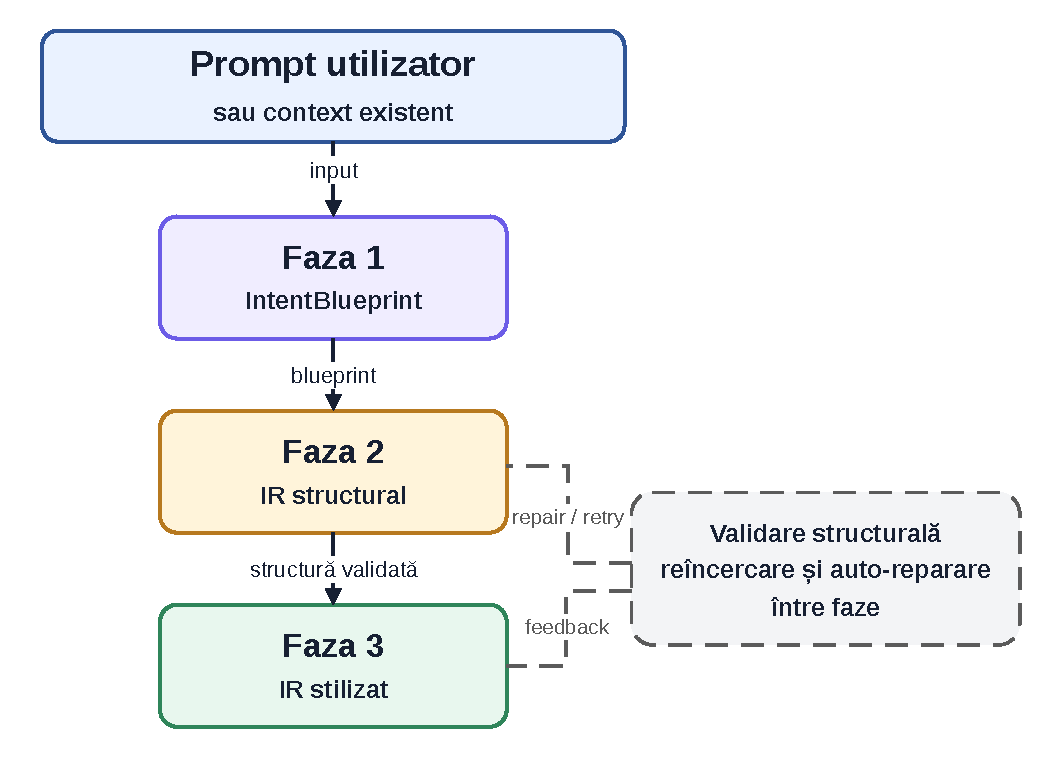
\includegraphics[width=0.80\textwidth]{diagrams/pipeline-ai.drawio.pdf}
  \caption{Pipeline-ul AI în trei faze folosit în Favigon}
  \label{fig:pipeline-ai}
\end{figure}

\section{Faza 1: extragerea intenției}

În prima etapă, sistemul nu încearcă să deseneze nimic și nu generează cod. Obiectivul este mai restrâns: să transforme promptul utilizatorului într-un \textit{IntentBlueprint}. În implementare, acest blueprint conține informații precum tipul paginii, starea vizuală generală, personalitatea brandului, publicul țintă, CTA-ul principal și lista secțiunilor în ordinea lor.

Acest pas explicit este important din două motive. În primul rând, el forțează modelul să ia o decizie de structură înainte să intre în detalii estetice. În al doilea rând, oferă frontend-ului și backend-ului o reprezentare intermediară ușor de afișat, inspectat sau discutat.

În practică, această etapă seamănă mai mult cu o analiză de cerințe decât cu o generare vizuală. Promptul este reinterpretat într-un format intern. Dacă utilizatorul cere, de exemplu, o pagină de prezentare pentru un produs SaaS, rezultatul nu trebuie să fie imediat un hero cu gradient, ci o listă de secțiuni și intenții: navbar, hero, beneficii, social proof, CTA, footer și așa mai departe.

\section{Faza 2: generarea structurii}

A doua etapă este cea care construiește efectiv arborele intermediar de noduri și reprezintă etapa centrală a întregii abordări. În loc să fie cerute modelului HTML final sau componente de framework, sarcina transmisă este producerea unui arbore `IRNode` cu layout, dimensiuni, padding, gap, poziționare și text.

Mai concret, structura generată include tipuri de noduri, copii, meta-informații, stiluri și reguli de layout. Promptul sistem pentru această fază este mult mai strict decât în prima etapă și include reguli explicite despre cum trebuie dimensionate secțiunile, cum trebuie folosite tipografiile, ce înseamnă `fit-content`, când se poate folosi `100%` și cum trebuie numite nodurile.

Această rigiditate este intenționată. Dacă în faza de intenție modelul are libertate mai mare, în faza structurală libertatea trebuie redusă. Altfel, ar exista prea multe variații greu de validat și greu de convertit.

\section{Faza 3: stilizarea}

A treia etapă pornește de la structura deja creată și aplică sistemul vizual: culori, gradiente, umbre, raze, borduri, cursor și alte detalii de prezentare. În implementare, promptul pentru această fază conține o regulă foarte importantă: layout-ul și structura nu trebuie modificate. Altfel spus, stilizarea nu are voie să rescrie ceea ce a rezolvat deja etapa de structură.

Această separare între structură și stil este utilă atât pentru control, cât și pentru depanare. Dacă o pagină este logică, dar arată slab, știu că problema este în faza a treia. Dacă layout-ul este greșit, știu că problema este în faza a doua. În plus, această abordare seamănă mai bine cu modul în care lucrează și oamenii: întâi decid structura și ierarhia, apoi rafinează aspectul vizual.

\section{Integrarea cu OpenAI API}

În Favigon, comunicarea cu modelul este abstractizată prin `OpenAiClient`. Acesta folosește endpoint-ul de \textit{Chat Completions} și suportă atât răspuns obișnuit, cât și streaming \cite{openaiChatCompletions2026}. Alegerea de a ascunde apelurile HTTP într-un adaptor de infrastructură păstrează serviciile de aplicație concentrate pe logică și face mai ușoară înlocuirea sau extinderea integrării în viitor.

Clientul construiește payload-ul cu mesaj de sistem, mesaj de utilizator, model configurabil și, unde este cazul, \texttt{response\_format} bazat pe schemă JSON. În plus, pentru scenariile de streaming, clientul parcurge liniile SSE și extrage incremental conținutul transmis de model. În implementarea actuală, identificatorul modelului este citit din configurație, cu fallback la \texttt{gpt-5.4-mini}, iar cererile trimit atât \texttt{response\_format}, cât și un prag explicit de \texttt{max\_completion\_tokens} pentru a limita comportamentul apelului la parametri observați și reproductibili.

Păstrarea identificatorului modelului în configurație, nu hardcodat în logică, este importantă deoarece partea experimentală a aplicației poate necesita ajustări de model în timp, iar aceste schimbări nu ar trebui să implice recompilarea serviciului de aplicație.

\section{Structura cererilor AI și feedback incremental}

Din punctul de vedere al API-ului, integrarea AI nu primește doar un simplu șir de text. Cererea de bază către endpoint-urile de design include promptul, un viewport țintă, modelul ales și, opțional, o structură IR existentă. Acest ultim câmp este important deoarece permite scenarii în care utilizatorul nu cere generarea unei pagini de la zero, ci rafinarea sau extinderea unei structuri deja existente. În cazul pipeline-ului pe trei faze, aceeași cerere mai include și parametrul \texttt{StopAfterPhase}, ceea ce face posibilă oprirea controlată după faza de intenție sau după faza structurală.

\begin{table}[H]
  \centering
  \caption{Câmpuri relevante din cererile AI folosite de backend}
  \label{tab:campuri-cereri-ai}
  \renewcommand{\arraystretch}{1.15}
  \begin{tabularx}{\textwidth}{>{\RaggedRight\arraybackslash}p{3.2cm}YY}
    \toprule
    \textbf{Câmp} & \textbf{Semnificație} & \textbf{Rol în procesare} \\
    \midrule
    \texttt{Prompt} & descrierea textuală a interfeței dorite & punctul de pornire pentru interpretarea intenției \\
    \texttt{ExistingIr} & structură intermediară existentă, opțională & permite extindere, reparare sau rafinare în loc de generare complet nouă \\
    \texttt{ViewportWidth} & lățimea de referință a paginii generate & influențează presupunerile de layout și scară \\
    \texttt{Model} & identificatorul modelului folosit & permite alegerea explicită între variantele configurate \\
    \texttt{StopAfterPhase} & limită de oprire pentru pipeline-ul în 3 faze & utilă pentru schițe parțiale, depanare și observarea etapelor intermediare \\
    \bottomrule
  \end{tabularx}
\end{table}

Suportul pentru streaming schimbă semnificativ și experiența utilizatorului. În loc să aștepte un singur răspuns final, frontend-ul poate primi evenimente incremental și poate afișa progresul procesării. În implementarea actuală, endpoint-urile de streaming trimit răspunsuri de tip \texttt{text/event-stream}, iar backend-ul emite linii SSE în care tipul evenimentului și conținutul sunt transmise separat. Pentru pipeline-ul în trei faze, evenimente precum \texttt{phase\_start}, \texttt{phase\_complete}, \texttt{result} sau \texttt{error} oferă o vizibilitate mult mai bună asupra procesului decât o simplă animație de încărcare.

\begin{lstlisting}[style=favigon,caption={Exemplu simplificat de evenimente SSE trimise în timpul pipeline-ului AI}]
event: phase_start
data: {"phase":1,"name":"intent"}

event: phase_complete
data: {"phase":1,"name":"intent"}

event: result
data: {"success":true,"stopAfterPhase":3}
\end{lstlisting}

Din punct de vedere operațional, fluxul complet dintre utilizator, frontend, controller, orchestration service și modelul AI este mai bine surprins printr-o diagramă de secvență. Figura~\ref{fig:secventa-ai} evidențiază atât schimburile principale de mesaje, cât și faptul că pipeline-ul nu este un singur apel, ci o succesiune controlată de faze cu feedback incremental.

\begin{figure}[H]
  \centering
  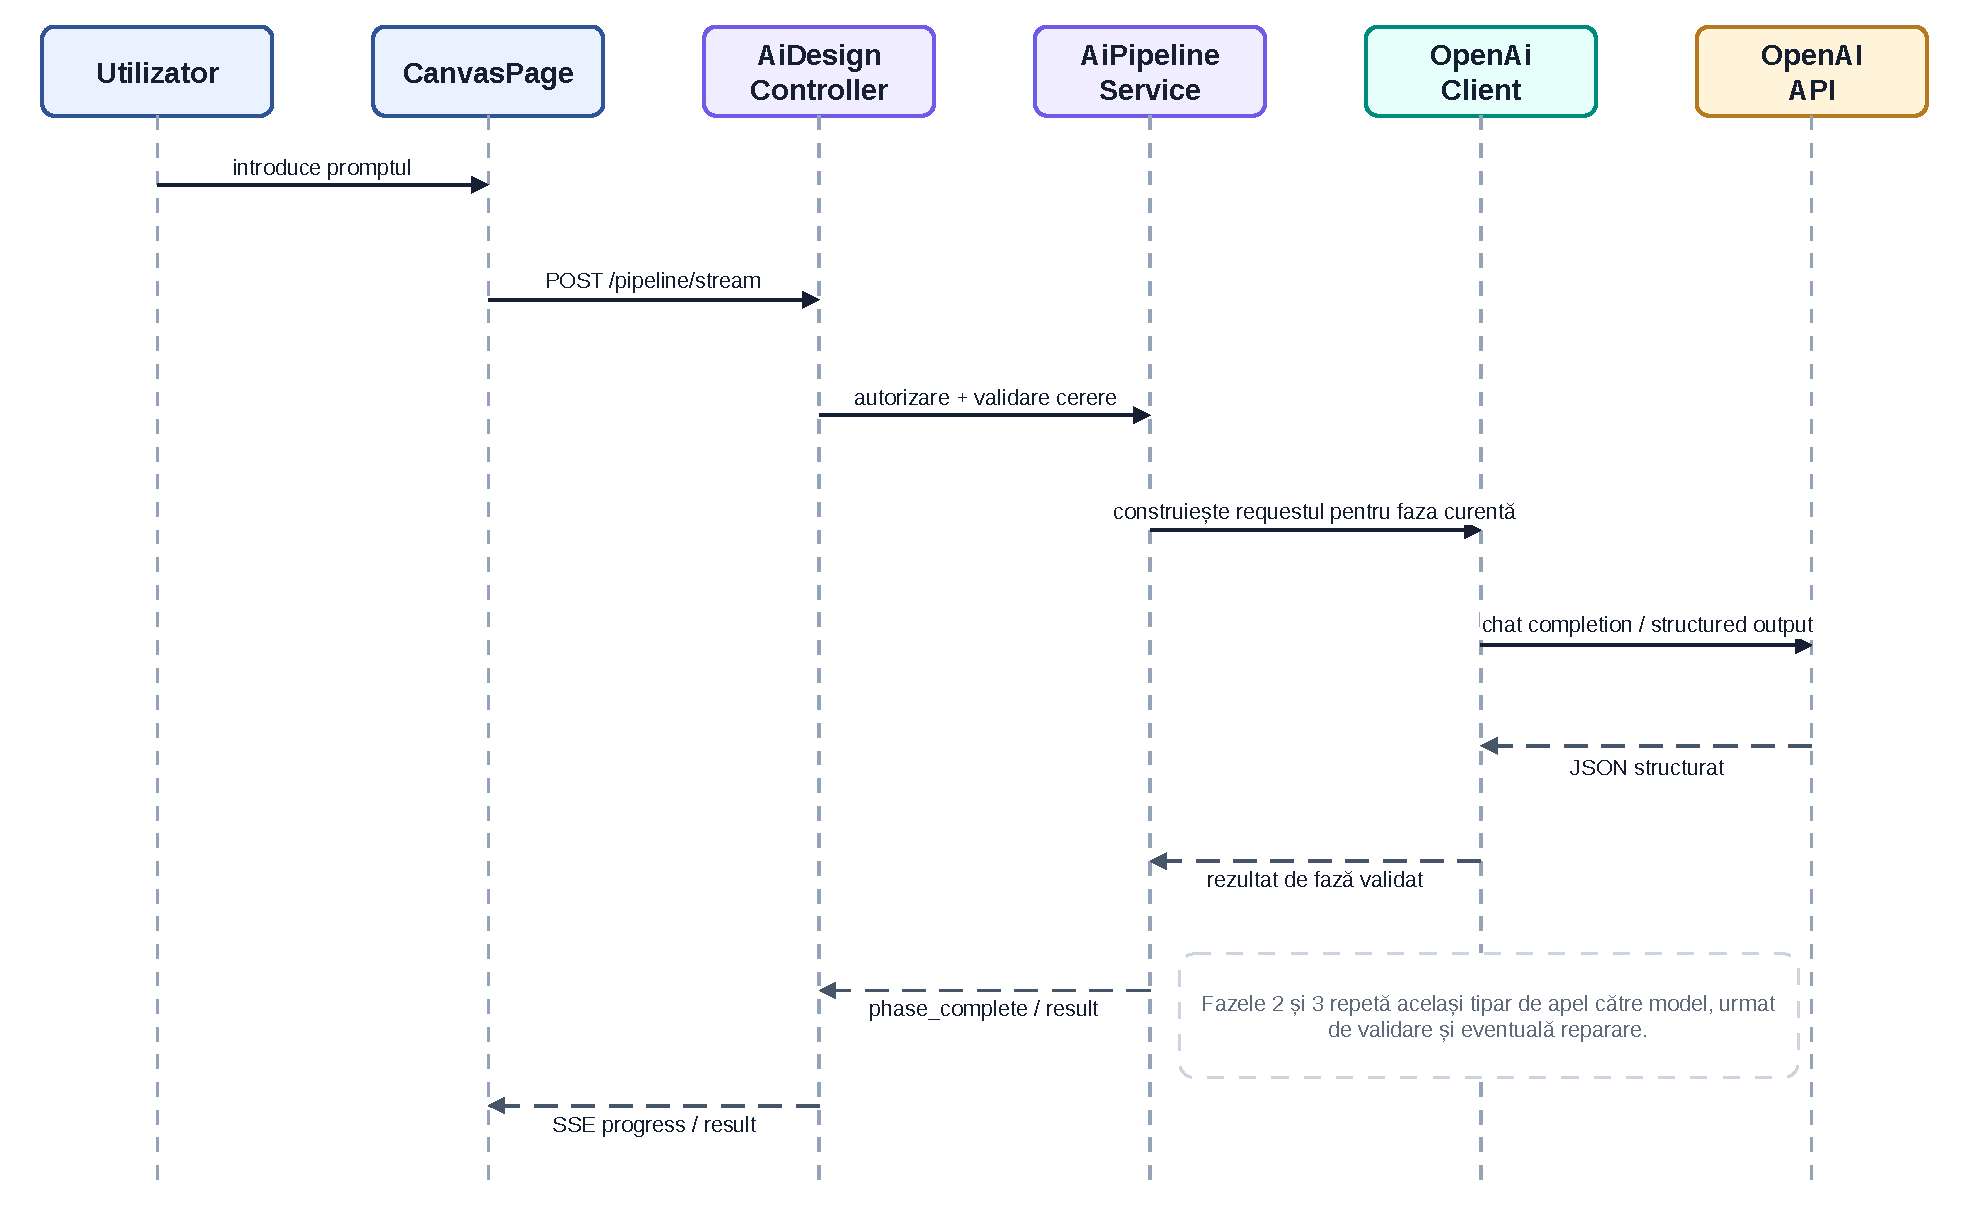
\includegraphics[width=\textwidth]{diagrams/secventa-ai.drawio.pdf}
  \caption{Diagrama de secvență simplificată pentru fluxul AI cu streaming}
  \label{fig:secventa-ai}
\end{figure}

\section{Rolul ieșirilor structurate}

OpenAI documentează explicit posibilitatea obținerii unor ieșiri structurate, conforme cu un anumit format sau cu o anumită schemă \cite{openaiStructuredOutputs2026}. În proiect, această capabilitate este foarte importantă. Dacă modelul ar întoarce doar text liber, parser-ul și validarea ar deveni mult mai fragile. În schimb, cu o schemă bine definită, aplicația poate detecta mai repede abaterile și poate decide dacă rezultatul este utilizabil sau nu.

Totuși, experiența din implementare arată că \textit{structured output} nu este o soluție magică. El ajută la format, dar nu garantează automat calitatea semantică a rezultatului. De exemplu, un JSON perfect valid poate descrie o structură slabă sau o ierarhie de secțiuni nepotrivită. Din acest motiv, `AiPipelineService` folosește atât deserializare și validare structurală, cât și reguli suplimentare și un pas de auto-reparare când rezultatul nu este acceptabil.

\section{Mecanisme de validare și reparare}

După fiecare etapă relevantă, rezultatul este analizat înainte să fie acceptat. Dacă în faza structurală arborele IR nu poate fi parsat sau nu respectă schema așteptată, serviciul încearcă un pas suplimentar de reparare. Acest pas trimite către model erorile de validare și o variantă trunchiată a rezultatului defect, cerând un JSON corectat.

Practic, modelul este tratat nu doar ca generator, ci și ca potențial asistent pentru repararea propriilor ieșiri. Această idee este utilă în contextul lucrării deoarece arată un mod mai realist de folosire a AI-ului: prima ieșire nu este presupusă perfectă, iar sistemul este proiectat explicit pentru a gestiona erori.

În plus, atât `AiDesignService`, cât și `AiPipelineService` folosesc cache cu TTL de 10 minute pentru cereri identice și validează separat răspunsurile obținute. În varianta de pipeline există și posibilitatea de oprire după faza 1 sau 2, respectiv emiterea de evenimente SSE de tip \texttt{phase\_start} și \texttt{phase\_complete}, ceea ce face procesul mai ușor de urmărit în interfață și în depanare.

\section{Reprezentarea intermediară în detaliu}

Structura `IRNode` este elementul care leagă editorul, AI-ul și convertorul. Un nod include identificator, tip, proprietăți, layout, stil, poziționare, copii, variante responsive, metadate și, opțional, efecte de animație. Această structură este suficient de generală pentru a descrie atât containere, cât și text, imagini sau frame-uri de pagină.

În practică, modelul intermediar oferă trei beneficii majore.

Primul este \textbf{independența față de framework}. Un `IRNode` nu este nici componentă Angular, nici JSX React, nici HTML final. De aceea poate fi transformat în toate aceste forme.

Al doilea este \textbf{validabilitatea}. Pentru că structura este explicită, poate fi verificată existența anumitor câmpuri, coerența layout-ului sau compatibilitatea dimensiunilor înainte de export.

Al treilea este \textbf{trasabilitatea}. Când ceva nu merge bine în export, structura intermediară poate fi inspectată și se poate vedea dacă problema vine din editor, din AI sau din convertor.

\section{Maparea dintre canvas și IR}

Pe partea de frontend, designul construit în editor nu este trimis direct către convertor în forma nativă a canvas-ului. În schimb, există mapper-e care transformă datele editorului în IR și invers. Acest detaliu este foarte important pentru arhitectura proiectului.

Dacă editorul ar fi legat direct de codul final, orice schimbare în convertor ar risca să rupă și logica din canvas. Prin introducerea mapper-elor, este creat un punct de decuplare. Editorul poate evolua într-o anumită direcție, iar convertorul în alta, atâta timp cât contractul IR rămâne coerent.

Maparea inversă, din IR în elemente de canvas, este la fel de utilă. Ea face posibilă integrarea rezultatelor generate de AI direct în editor, astfel încât utilizatorul să nu primească un export static, ci un design pe care îl poate modifica în continuare.

\section{Exemplu concret de flux de la prompt la IR și export}

Pentru a înțelege mai clar legătura dintre subsisteme, este util un exemplu simplificat. Presupunând un prompt de tipul „creează o pagină landing pentru o aplicație de task management, cu hero, beneficii și call-to-action”, prima fază nu produce HTML și nici noduri finale, ci o descriere structurată a intenției: tip de pagină, audiență, ton vizual și secțiuni în ordinea așteptată. A doua fază transformă această intenție într-un arbore IR cu frame principal, containere, text și butoane, iar a treia aplică stilurile. Abia după aceste etape structura ajunge la convertor.

În etapa de export, convertorul primește fie un singur \texttt{IRNode}, fie o listă de pagini. Pentru cazul simplu single-page, \texttt{ConverterController} apelează validarea și apoi \texttt{Generate}. Pentru cazul multi-page, aceeași rută de generare poate primi \texttt{Pages}, iar endpoint-ul dedicat pentru fișiere folosește \texttt{GenerateMultiPage}. Rezultatul nu este doar o bucată de cod brut, ci un set coerent de artefacte adaptate framework-ului cerut: HTML și CSS pentru varianta statică, respectiv fișiere de componentă, stil și structură pentru React sau Angular.

Acest exemplu arată de ce separarea pe etape este importantă. Dacă problema apare în secționarea paginii sau în ierarhia elementelor, ea poate fi localizată înainte de convertor. Dacă structura este corectă, dar codul rezultat nu respectă așteptările, zona de investigație se mută în motorul de export. În practică, această trasabilitate reduce mult costul depanării și face sistemul mai explicabil în comparație cu o abordare directă „prompt în, cod afară”.

\section{Motorul de conversie}

\subsection{Separarea în proiect dedicat}

Motorul de conversie este implementat în proiectul `Favigon.Converter`. El este separat explicit de `Favigon.Application` deoarece are propria logică de validare, transformare și emitere. Dacă ar fi rămas îngropat în același serviciu cu restul aplicației, ar fi fost mai greu de testat și mai greu de extins.

\subsection{Validarea}

Înainte de generare, `ConverterService` cere motorului verificarea structurii IR. Dacă apar erori, ele sunt raportate și procesul se oprește. Această etapă este necesară pentru că ieșirea finală ar deveni altfel imprevizibilă. Este preferabil refuzul unui export decât generarea de cod inconsistent fără semnalarea problemei.

\subsection{Generarea single-page și multi-page}

`ConverterEngine` suportă atât generarea pentru o singură pagină, cât și generarea pentru mai multe pagini. Pentru multi-page, motorul produce seturi de fișiere și gestionează numele de pagini, slug-urile și structura finală. În cazul exportului Angular sau React, el generează și fișiere de proiect minimal, rute și fișiere CSS.

Această capabilitate este importantă deoarece proiectul nu se reduce la o singură artboard. Odată ce editorul suportă mai multe pagini, exportul trebuie să poată păstra această structură.

\begin{figure}[H]
  \centering
  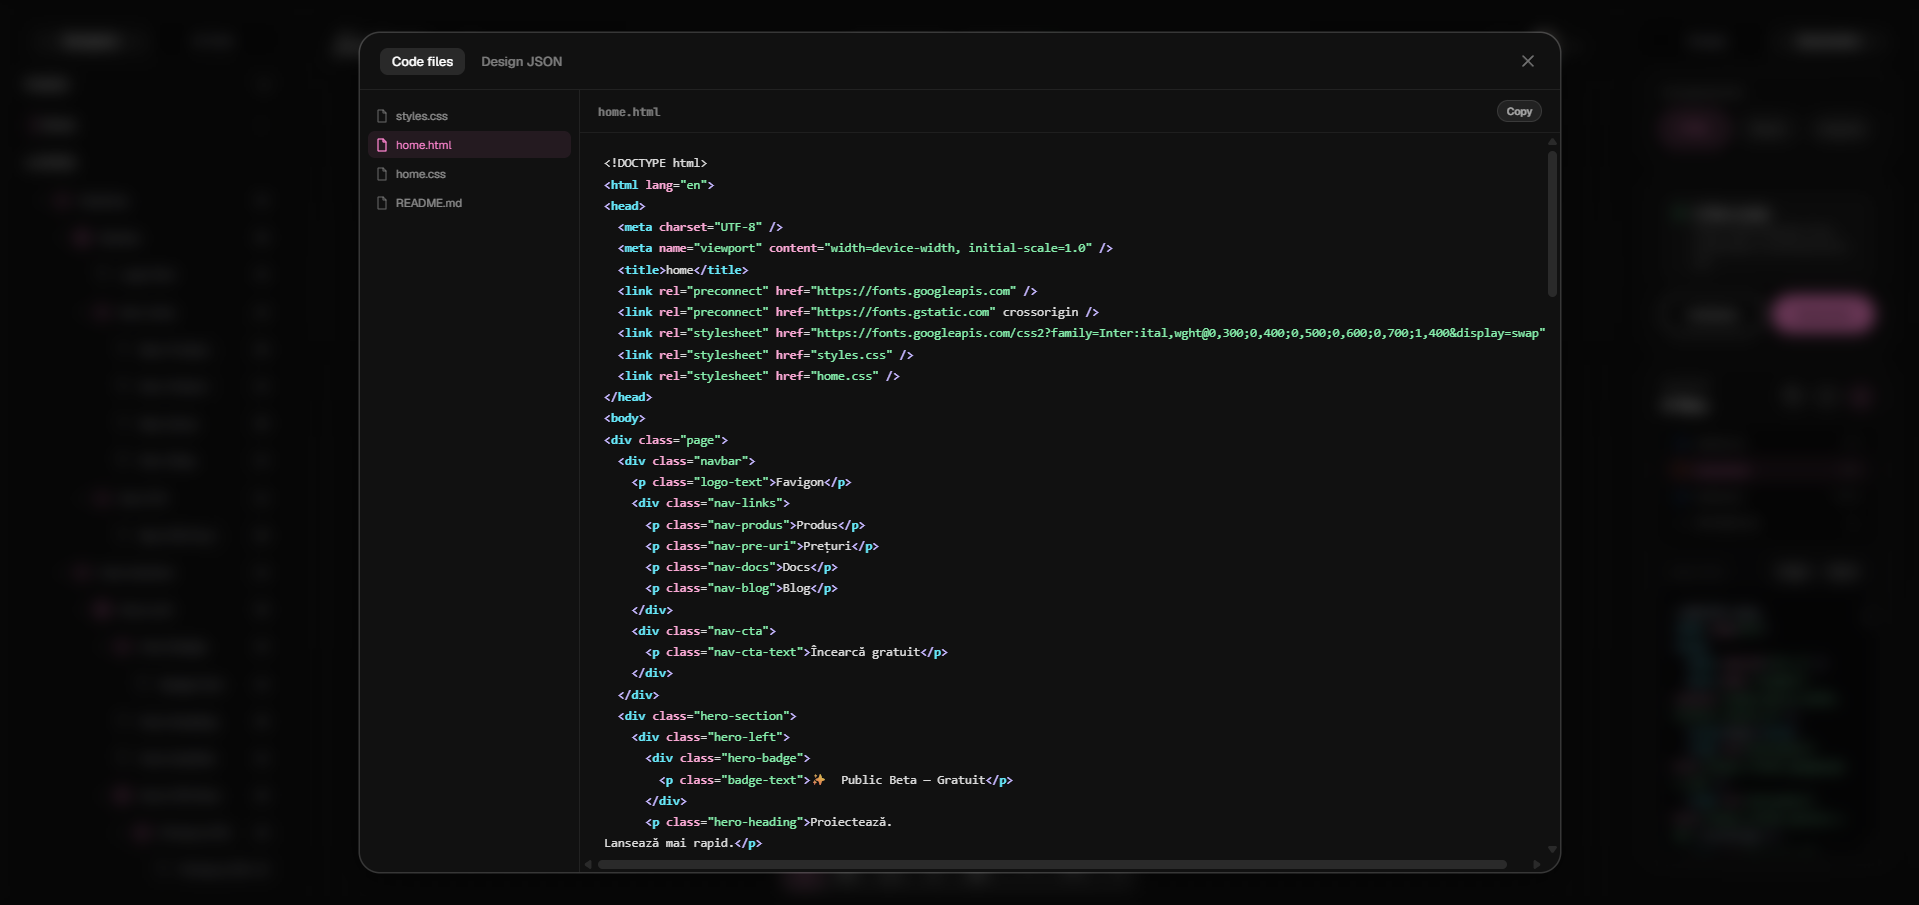
\includegraphics[width=0.94\textwidth]{images/generated_code.png}
  \caption{Exemplu de artefacte generate și inspectate în interfața de export}
  \label{fig:generated-code}
\end{figure}

\subsection{Responsive output}

O componentă mai tehnică și mai interesantă este exportul responsive. În loc să dublez pur și simplu tot arborele pentru fiecare breakpoint, motorul produce artefactele principale și apoi diferențe CSS pentru breakpoints suplimentare. În testele existente se vede că sunt tratate cazuri precum noduri prezente doar pe anumite breakpoint-uri, schimbări de ordine pentru copii flex și diferențe de pseudo-clase sau keyframes.

Aceasta este una dintre funcțiile care arată cel mai clar că proiectul nu se oprește la un export superficial. Există o preocupare reală pentru cum este construit rezultatul final și pentru cât de mult poate fi controlat. Fluxul complet canvas $\rightarrow$ IR $\rightarrow$ artefacte de export este rezumat în Figura~\ref{fig:design-to-code}.

\begin{figure}[H]
  \centering
  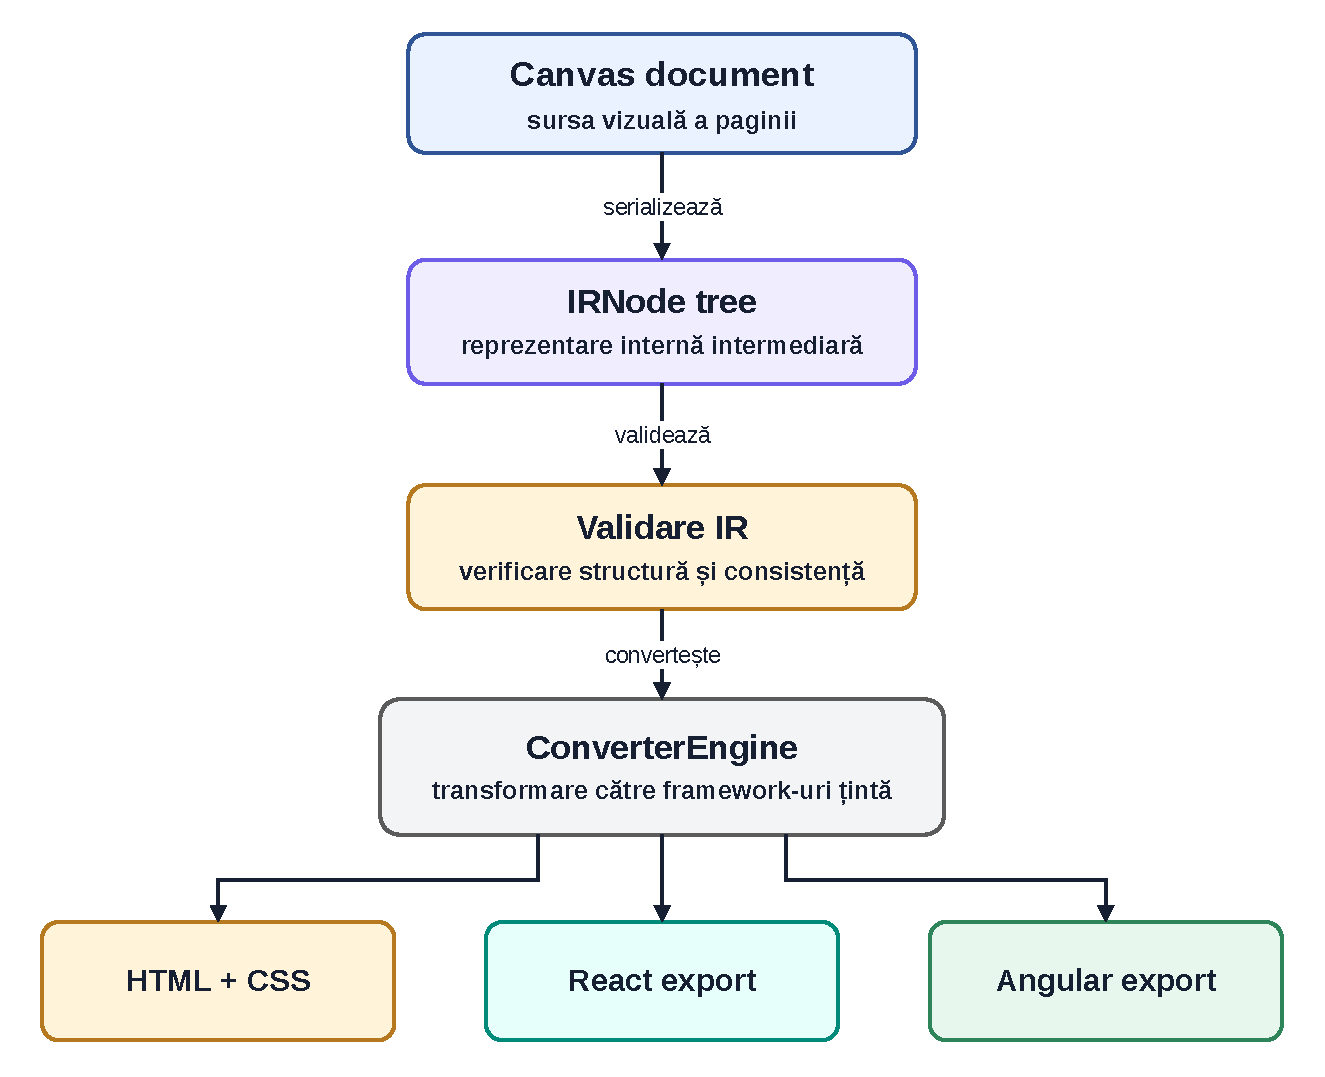
\includegraphics[width=0.90\textwidth]{diagrams/design-to-code.drawio.pdf}
  \caption{Fluxul design-to-code bazat pe reprezentarea intermediară}
  \label{fig:design-to-code}
\end{figure}

\section{Legătura dintre AI și convertor}

Un aspect foarte important este faptul că AI-ul și convertorul nu sunt două subsisteme complet separate. Ele comunică prin aceeași reprezentare intermediară. Fără această alegere, rezultatul generat de AI ar fi fost mult mai greu de transformat în cod într-un mod controlat.

Pe scurt, pipeline-ul AI generează un arbore care este suficient de bogat pentru a fi editat și suficient de formal pentru a fi convertit. În momentul în care această condiție este îndeplinită, editorul devine interfața de rafinare, iar convertorul devine ieșirea tehnică. Această relație dintre cele trei module --- AI, editor și convertor --- reprezintă contribuția tehnică principală a întregului proiect.

\section{Limitări actuale}

Deși soluția funcționează și este coerentă, există și limite.

În primul rând, calitatea rezultatului AI depinde încă mult de prompt și de regulile incluse în mesajele de sistem. Cu alte cuvinte, caracterul probabilistic al modelului nu este eliminat; el este doar controlat mai bine.

În al doilea rând, reprezentarea intermediară este suficient de bogată pentru scopurile actuale, dar nu acoperă toate situațiile pe care le-ar avea un constructor comercial matur. De exemplu, colaborarea în timp real, constrângerile mai avansate de componentizare sau integrarea automată cu design systems externe ar necesita extinderi suplimentare.

În al treilea rând, exportul generat este orientat spre claritate și portabilitate, nu neapărat spre cele mai sofisticate convenții ale fiecărui ecosistem. Pentru o platformă academică, acest compromis este acceptabil.

\section{Concluzii intermediare}

Capitolul de față descrie partea cea mai originală din proiect. Generarea asistată de AI nu este tratată ca un artificiu separat, ci ca parte a unei arhitecturi care include reprezentare intermediară, validare, reparare și conversie în cod. Tocmai această integrare controlată face diferența între o demonstrație izolată și un produs software coerent.

În capitolul următor sunt urmărite scenarii concrete de utilizare, pentru a observa cum colaborează în practică editorul, AI-ul, preview-ul, exportul și componenta socială. Abia după această etapă este discutată explicit validarea sistemului prin măsuri de securitate și testare.


